\documentclass[a4paper,UTF8]{ctexart}

\usepackage{amsmath, amsthm, amssymb, amsfonts, hyperref, mathrsfs}%美国数学学会的包+?
\usepackage{geometry} %控制界面
\usepackage{bookmark}
\usepackage{fancyhdr} % header & footer
\usepackage{appendix} % 附录
\usepackage{tikz} %作图
\usepackage{graphicx} %插入图片的宏包
\usepackage{float} %设置图片浮动位置的宏包
%\usepackage{subfigure} %插入多图时用子图显示的宏包
\usepackage{listings} %引用代码
\usepackage{physics,mathtools} %物理数学工具
\usepackage{comment}
\usepackage{framed}
\usepackage{caption}
\usepackage{subcaption}
\geometry{top=2.5cm,bottom=2.5cm,left=2.5cm,right=2.5cm} % 布局要求
\pagestyle{fancy} % fancy分格
\fancyhf{} % 清除所有页眉页脚
\renewcommand\headrulewidth{0.6pt}
\renewcommand\footrulewidth{0.6pt}
% font
\setCJKmainfont{Noto Serif CJK SC}[BoldFont={Noto Serif CJK SC Bold}, ItalicFont=]
\lhead{何金铭 PB21020660$\mid$座位号:5}
\chead{量子计算实验报告}
\rhead{\thepage}
\lfoot{2024.4.12}
\rfoot{USTC}
%\bibliographystyle{plain} % 引用样式
\everymath{\displaystyle} % display
%============================================================

\begin{document}

\begin{center}
    \textbf{\Large 量子计算实验报告}
    \par \text{\large 何金铭 PB21020660}
\end{center}

实验目的,实验原理,实验内容已于预习报告中给出,此处不再赘述。

\section{实验结果与分析}

\subsection{连续波实验}

当波源功率为3dBm时,测得的连续波谱如下:

\begin{figure}[H]
    \centering
    \begin{minipage}[b]{0.9\textwidth}
        \centering
        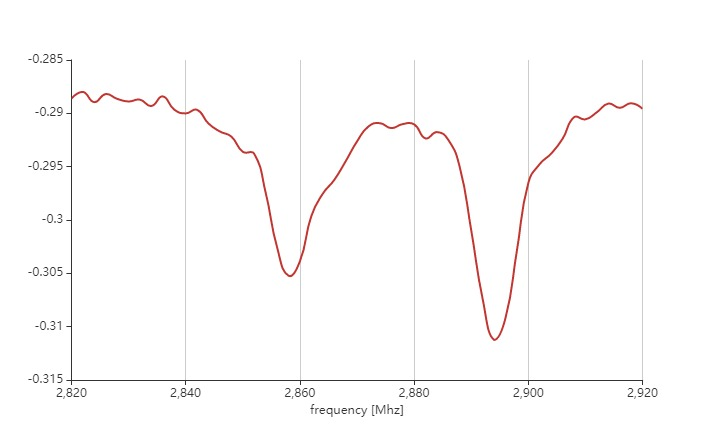
\includegraphics[width=0.85\textwidth]{./1.jpeg}
        \caption{波源功率为3dBm时的连续波谱}
    \end{minipage}
\end{figure}

两个吸收峰分别为2894MHz和2858MHz。

当波源功率为-6dBm时,测得的连续波谱如下:

\begin{figure}[H]
    \centering
    \begin{minipage}[b]{0.9\textwidth}
        \centering
        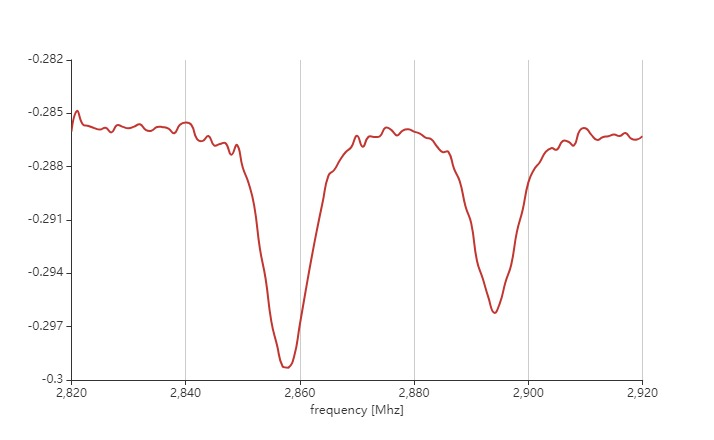
\includegraphics[width=0.85\textwidth]{./2.jpeg}
        \caption{波源功率为-6dBm时的连续波谱}
    \end{minipage}
\end{figure}

两个吸收峰分别为2894MHz和2858MHz,之前一致。

可知$\ket{0}$与$\ket{-1}$间的能级差为2858MHz,$\ket{0}$与$\ket{1}$间的能级差为2894MHz。

\subsection{Rabi震荡实验}

\subsubsection{微波频率为2894MHz,波源功率为3dBm}


\begin{figure}[H]
    \centering
    \begin{minipage}[b]{0.9\textwidth}
        \centering
        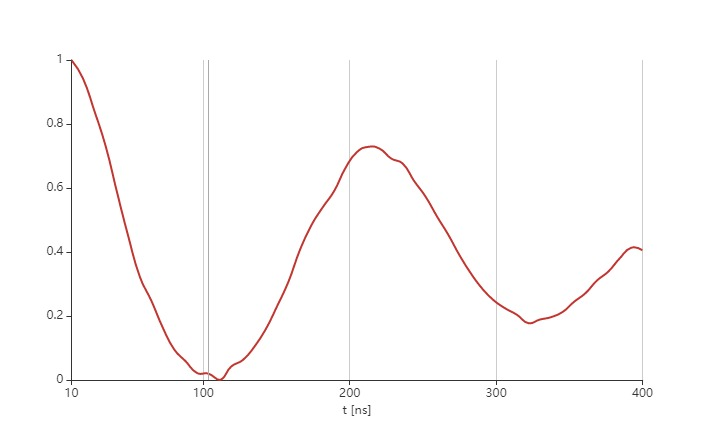
\includegraphics[width=0.85\textwidth]{./3.jpeg}
        \caption{微波频率为2894MHz,波源功率为3dBm时的拉比震荡}
    \end{minipage}
\end{figure}

测得$t_{\frac{\pi}{2}} = 45ns, t_{\pi} = 105ns,t_{2\pi} = 210ns$

\subsubsection{微波频率为2858MHz,波源功率为3dBm}   

\begin{figure}[H]
    \centering
    \begin{minipage}[b]{0.9\textwidth}
        \centering
        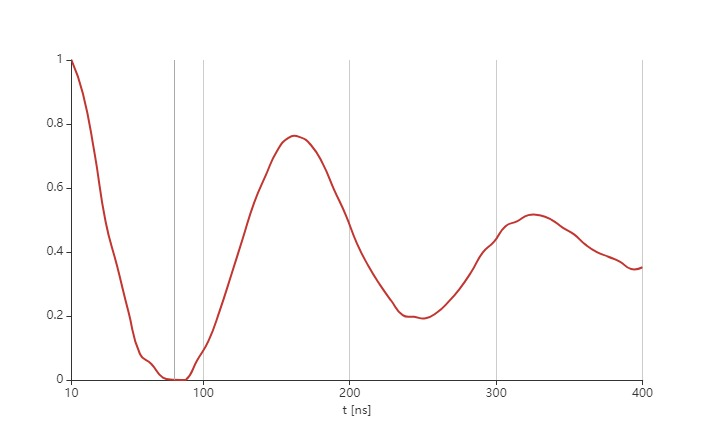
\includegraphics[width=0.85\textwidth]{./4.jpeg}
        \caption{微波频率为2858MHz,波源功率为3dBm时的拉比震荡}
    \end{minipage}
\end{figure}

$t_{\frac{\pi}{2}} = 41.2ns, t_{\pi} = 80ns,t_{2\pi} = 160ns$

\subsubsection{微波频率为2858MHz,波源功率为6dBm}   

\begin{figure}[H]
    \centering
    \begin{minipage}[b]{0.9\textwidth}
        \centering
        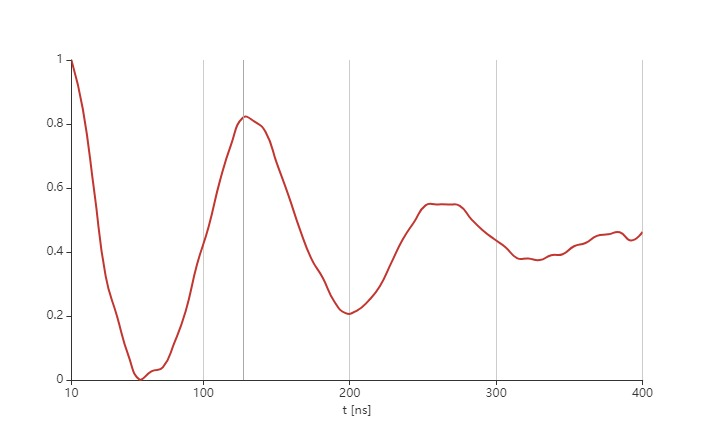
\includegraphics[width=0.85\textwidth]{./5.jpeg}
        \caption{微波频率为2858MHz,波源功率为6dBm时的拉比震荡}
    \end{minipage}
\end{figure}

$t_{\frac{\pi}{2}} = 30ns, t_{\pi} = 60ns,t_{2\pi} = 127ns$

\subsection{回波实验}

\begin{table}[H]
    \centering
    \caption{回波实验参数设置表}
    \begin{tabular}{|l|l|l|l|}
    \hline
        微波频率 MHz & 微波功率 dBm & pi脉冲宽度 ns & pi/2脉冲宽度 ns \\ \hline
        2894 & 3 & 105 & 45 \\ \hline
    \end{tabular}
\end{table}

\begin{figure}[H]
    \centering
    \begin{minipage}[b]{0.9\textwidth}
        \centering
        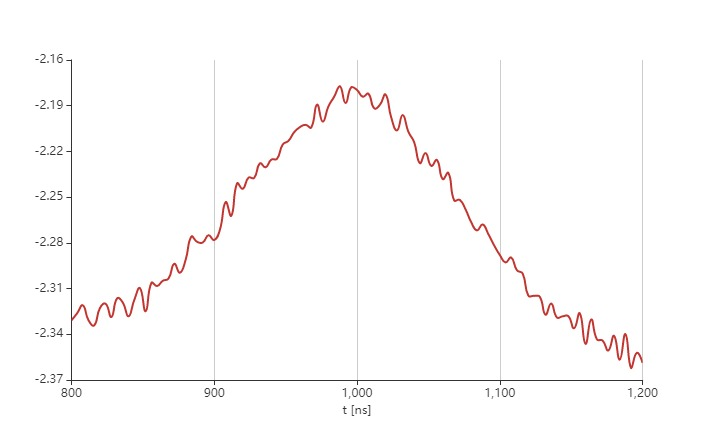
\includegraphics[width=0.85\textwidth]{./6.jpeg}
        \caption{微波频率为2894MHz,波源功率为3dBm时的回波实验}
    \end{minipage}
\end{figure}

可以观察到一个明显左右对称的回波信号,回波信号大致为1000ns长。

\subsection{$T_2$实验}

\begin{table}[H]
    \centering
    \caption{$T_2$实验参数设置表}
    \begin{tabular}{|l|l|l|l|}
    \hline
        微波频率 MHz & 微波功率 dBm & pi脉冲宽度 ns & pi/2脉冲宽度 ns \\ \hline
        2894 & 3 & 105 & 45 \\ \hline
    \end{tabular}
\end{table}

实验测得的结果为:

\begin{figure}[H]
    \centering
    \begin{minipage}[b]{0.9\textwidth}
        \centering
        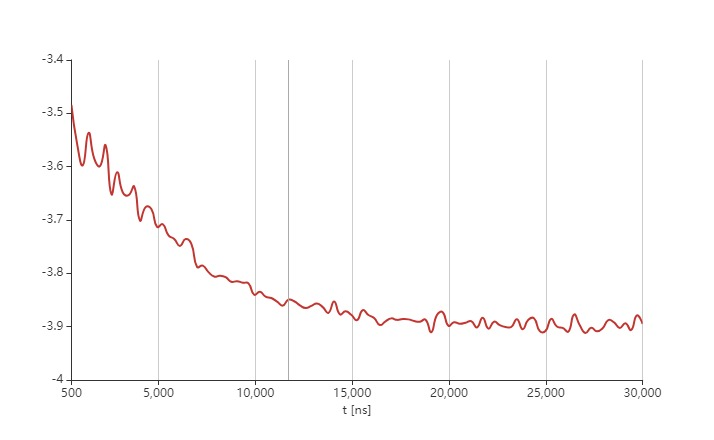
\includegraphics[width=0.85\textwidth]{./7.jpeg}
        \caption{微波频率为2894MHz,波源功率为3dBm时的$T_2$实验}
    \end{minipage}
\end{figure}

带入拟合函数$f=A\cdot\exp(-(t/T_2)^a)+B$拟合得:

\begin{figure}[H]
    \centering
    \begin{minipage}[b]{0.9\textwidth}
        \centering
        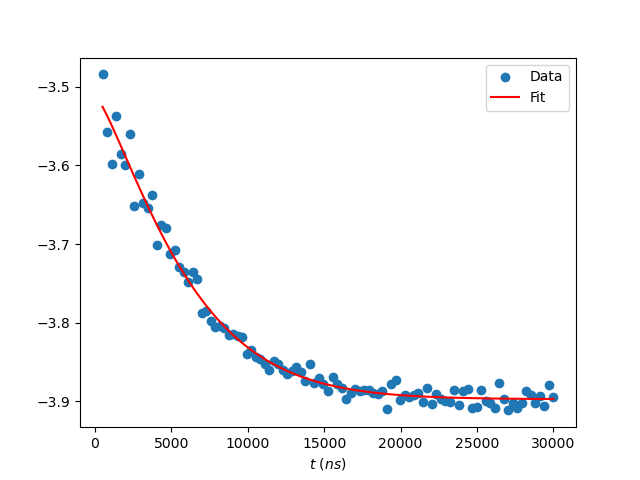
\includegraphics[width=0.85\textwidth]{./1.png}
        \caption{微波频率为2894MHz,波源功率为3dBm时的$T_2$实验拟合结果}
    \end{minipage}
\end{figure}

并计算得拟合参数为:$A = 0.387, T_2 = 6412.16ns, a = 1.283, B = -3.898$

在实验中的时间参数均小于$T_2$,在相干时间内,故可以实现量子计算。

\subsection{D-J算法实验}

其他参数的设置与之前的结果设置,下面强调几点需要关注的参数:

\begin{enumerate}
    \item DJ1, DJ2参数的设置中微波1和微波2的波源功率均为3dBm;而DJ3, DJ4的参数设置中微波1的波源功率均为3dBm,微波2的波源功率为6dBm。这是因为微波2的转换效率小于微波1,而DJ3, DJ4的回波信号主要来自于微波2,故需要增加功率。
    \item DJ2, DJ4参数的设置中微波1的回波信号时间应设置为1210ns, 这是由于在DJ2, DJ4算法的回波时间中又设置了一个$2\pi$脉冲信号,故为$1210ns$;而DJ1, DJ3中只有一个回波信号,回波时间设置为$1000ns$
\end{enumerate}

\begin{figure}[H]
    \centering
    \begin{minipage}[b]{0.9\textwidth}
        \centering
        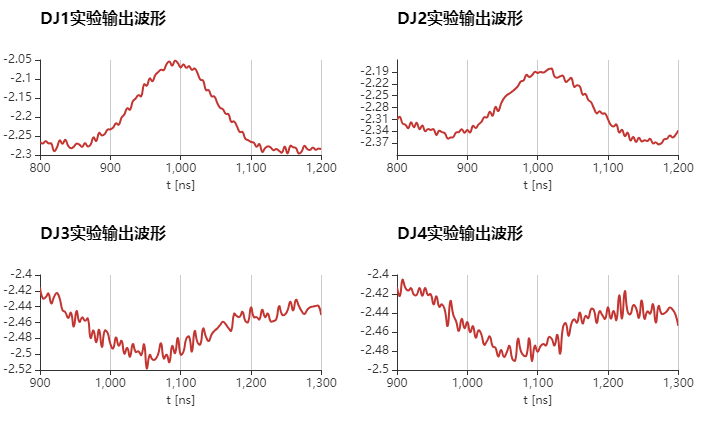
\includegraphics[width=1\textwidth]{./8.jpeg}
        \caption{DJ算法实验}
    \end{minipage}
\end{figure}

常函数的回波信号向上,而平衡函数的回波信号向下,故DJ1,DJ2的结果为常函数,DJ3,DJ4的结果为平衡函数。

\section{实验结论}

\begin{enumerate}
    \item 可知$\ket{0}$与$\ket{-1}$间的能级差为2858MHz,$\ket{0}$与$\ket{1}$间的能级差为2894MHz
    \item 微波频率为2894MHz,波源功率为3dBm时的拉比震荡,测得$t_{\frac{\pi}{2}} = 45ns, t_{\pi} = 105ns,t_{2\pi} = 210ns$;
    微波频率为2858MHz,波源功率为3dBm时的拉比震荡,$t_{\frac{\pi}{2}} = 41.2ns, t_{\pi} = 80ns,t_{2\pi} = 160ns$
    微波频率为2858MHz,波源功率为6dBm时的拉比震荡,$t_{\frac{\pi}{2}} = 30ns, t_{\pi} = 60ns,t_{2\pi} = 127ns$
    \item 测得微波1,2894MHz,3dBm的回波信号时间约为$1000ns$
    \item 测得微波1,2894MHz,3dBm的$T_2$信号时间为$T_2 = 6412.16ns$,在实验中的时间参数均小于$T_2 = 6412.16ns$,在相干时间内,故可以实现量子计算。
    \item DJ算法测试得:DJ1,DJ2的结果为常函数,DJ3,DJ4的结果为平衡函数。
\end{enumerate}

\section{思考题}

\subsection{请利用布洛赫球表示以下量子态:}

\begin{align}
    (1) |\psi\rangle=\frac{|0\rangle+|1\rangle}{\sqrt{2}} = \cos{45^{\circ}} \ket{0} + \sin{45^{\circ} \ket{1} \sim (\theta = 90^{\circ},\phi = 0)}\\
    (2) |\psi\rangle=\frac{|0\rangle-|1\rangle}{\sqrt{2}} = \cos{45^{\circ}} \ket{0} - \sin{45^{\circ} \ket{1} \sim (\theta = 90^{\circ},\phi = \pi)}\\
    (3) |\psi\rangle=\frac{|0\rangle+i|1\rangle}{\sqrt{2}} = \cos{45^{\circ}} \ket{0} + i \sin{45^{\circ} \ket{1} \sim (\theta = 90^{\circ},\phi = \frac{1}{2}\pi)}\\
    (4) |\psi\rangle=\frac{|0\rangle-i|1\rangle}{\sqrt{2}} = \cos{45^{\circ}} \ket{0} - i \sin{45^{\circ} \ket{1} \sim (\theta = 90^{\circ},\phi = \frac{3}{2}\pi)}
\end{align}

\subsection{如果实验中施加的微波频率$f$与共振频率$f_0$有偏差,即$f=f_0+\delta f$,拉比振荡的频率会如何变化?}

拉比震荡的频率为:

\begin{equation}
    \Omega = \sqrt{f_1^2 + (f- f_0)^2} = \sqrt{f_1^2 + \delta f^2}
\end{equation}

可知偏差越大震荡频率越大,但与此同时振幅也在减小.最后振幅小于一定值或者频率大于一定值时就无法分辨.

\subsection{拉比振荡频率与微波功率的关系是什么?}

由本实验中的Rabi震荡实验可得,当微波功率增大时,拉比振荡频率也会增大.
如图3,图5所示

一般情况下,微波功率的增加可以影响拉比振荡的频率,通常表现为以下两种情况:

\begin{enumerate}
    \item 线性关系:在一定范围内,拉比振荡频率与微波功率呈线性关系。当微波功率增加时,拉比振荡频率也相应增加。这种关系通常在微波功率较低的情况下成立,即微波功率尚未达到饱和效应(saturation)
    \item 饱和效应:当微波功率进一步增加时,拉比振荡频率将逐渐趋于饱和,即增加微波功率不再显著增加拉比振荡频率。这是因为在高功率下,系统的能级分布和激发态的寿命等因素会导致饱和效应的出现。此时,拉比振荡频率将趋于一个饱和值,不再随微波功率的增加而线性增加。
\end{enumerate}

本实验中大致属于线性关系.

\subsection{参照$n=1$的特殊情况,即图1.5所示的量子线路图,画出一般情况的D-J算法量子线路图,并解释算法原理。}

\begin{figure}[H]
    \centering
    \begin{minipage}[b]{0.9\textwidth}
        \centering
        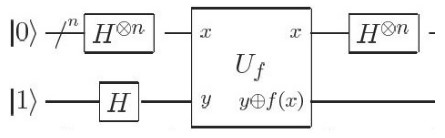
\includegraphics[width=0.6\textwidth]{./1.jpg}
        \caption{一般情况的DJ算法}
    \end{minipage}
\end{figure}

 已知$U_f$的$f(x)$只有两种可能,一种对$\forall x$为常数,一种对$\forall x$得到0、1的数目相同.

输入$|0\rangle^n|1\rangle$

计算得输出$\sum_z\sum_x\frac{(-1)^{f(x)+x\cdot z}|z\rangle}{2^n}\frac{|0)-|1\rangle}{\sqrt2}=\left\{\begin{array}{lll}|0\rangle^n\frac{|0\rangle-|1\rangle}{\sqrt2}&\text{,f(x)为常数}\\\sum_{z\neq[0]}\sum_x\frac{(-1)^{f(x)+x\cdot z}|z|}{2^n}\frac{|0)-|1\rangle}{\sqrt2}&\text{,f(x)为平衡}\end{array}\right. .$

测量前n个比特,若全部为0则f(x)为常数,若存在1则f(x)为平衡

\end{document}